
\documentclass[usletter, 10pt, conference]{ieeeconf}
\newcommand{\mbm}[1]{\mbox{\boldmath $#1$}}
\newcommand{\norm}[1]{\lVert#1\rVert}
\newcommand{\superscript}[1]{\ensuremath{^{\textrm{#1}}}}
\newcommand\blfootnote[1]{%
  \begingroup
  \renewcommand\thefootnote{}\footnote{#1}%
  \addtocounter{footnote}{-1}%
  \endgroup
}
\usepackage{url}

\usepackage[ruled]{algorithm2e}
\usepackage{subfigure}
\usepackage{graphicx,color,psfrag}
\usepackage{amsmath}
\usepackage{amsfonts}
\usepackage{amssymb}
\usepackage{bigdelim}
\usepackage{dsfont}
\usepackage{color, soul}
%\usepackage[section]{placeins}
%\usepackage{graphicx}
%\usepackage{caption}
%\usepackage{subcaption}

\overrideIEEEmargins
\title{The Autonomous Picking \& Palletizing (APPLE) Robot:\\ A Research Platform for
  Intralogistics Applications} 

% Multiple authors
\author{ \authorblockN{Robert Krug\superscript{*}, Todor Stoyanov\superscript{*}, Vinicio
    Tincani\superscript{\ddag}, Henrik Andreasson\superscript{*},\\ Rafael Mosberger\superscript{*},
    Gualtiero Fantoni\superscript{\ddag}, Achim J. Lilienthal\superscript{*} and Antonio
    Bicchi\superscript{\ddag}}
 %\authorblockA{\superscript{*}AASS Research Center, {\"O}rebro University, Sweden}
}

\begin{document}
\maketitle
\thispagestyle{empty}
\pagestyle{empty}
%
\blfootnote{\hspace{-4.5mm} \superscript{*} AASS Research Center; {\"O}rebro University; Studentgatan 1, 70182 {\"O}rebro, Sweden.\\
  \superscript{\ddag} Interdepart. Research Center ``E. Piaggio''; University of Pisa, Via Diotisalvi 2, 56100 Pisa, Italy.}
%
\begin{abstract}
  In this work we present a research platform for fully autonomous commissioning tasks in
  intralogistics settings. The robot comprises a nonholonomic mobile base and a manipulation system
  consisting of a lightweight arm and an under-actuated gripper with active surfaces. The platform
  is capable of autonomously picking up pallets and loading them with unstructured goods in a manner
  which is safe for human workers sharing the environment. Target object handling is accomplished
  via a novel, redundant grasp representation which allows for redundancy in the gripper pose
  placement. This redundancy is exploited by an optimization-based control system which generates
  reactive manipulator motions on-the-fly without the delays occurring in sense-plan-act
  architectures.
\end{abstract}
%
\section{Introduction}
\label{sec:intro}
%
The increasing need for fast and flexible commissioning ($i.\,e.,$ order picking and collection of
unstructured goods from storage compartments in warehouses) in logistic scenarios has created
substantial interest for autonomous robotic solutions. One of the main arguments for automating this
task is that the dull and strenuous nature of commissioning could cause mental and physical illness
in human workers. As a result, the determination within the logistics sector to invest in this area
is high and substantial efforts are made for the humanization of workstations~\cite{Eche08}.

There exist partial solutions for the automated commissioning problem in controlled
environments. The system described in~\cite{Wurm08} coordinates a fleet of Autonomous Ground
Vehicles (AGVs) which transport shelves filled with goods to a human worker who picks the
corresponding objects to complete the order. Key obstacles for a fully automatized solution
applicable in general warehouse settings are safe autonomous vehicle navigation in industrial
environments co-populated by humans, as well as the autonomous grasping/manipulation of unstructured
goods at satisfactory cycle times.
%
\begin{figure}[t!]
\begin{center}
\includegraphics[width =0.8\linewidth]{figs/apple_demonstrator}
%\vspace{-0.25cm}
\caption{\textit{The APPLE platform:} A KUKA LBR iiwa arm (3) is mounted on a retrofitted Linde
  CitiTruck AGV (7). For localization, a Velodyne HDL-32 Lidar (4) is used, human co-workers are
  detected with our RefleX camera system (6) presented in~\cite{Mosb14}. In order to detect pallets,
  we employ an Asus Xtion Pro Live structured light camera (5). The depicted grasping device (2) is
  a further developed and smaller version of the underactuated Velvet Fingers gripper described
  in~\cite{Tinc12}. Each of the gripper’s two fingers has a planar manipulator structure with two
  rotary joints and active surfaces which are implemented by conveyor belts on the inside of the two
  phalanges. These belts are used to assist in robust grasp acquisition as described in
  \mbox{Section~\ref{subsec:grasp_execution}}. Object detection is done with a Structure IO device
  (1) which is mounted on the gripper's palm.}
\label{fig:robot}
\vspace{-0.65cm}
\end{center}
\end{figure}

In this work, we present the Autonomous Picking \& Palletizing (APPLE) research platform (see
Fig.~\ref{fig:robot}) which we developed to address the following important sub-task chain which
occurs during commissioning in prototypical warehouses: autonomous picking of goods from a storage
location, subsequent placement on a standard EUR pallet and transport of the filled pallet to a
target location. Furthermore, this process has to be carried out in a manner which is safe for
humans operating in the same environment. The platform's mobile base consists of a retrofitted
nonholonomic Linde CitiTruck forklift AGV\footnote{\url{ http://www.citi-truck.com}} which is able
to detect and pick up pallets in designated loading zones. A KUKA LBR
iiwa\footnote{\url{http://www.kuka-labs.com/en/service_robotics/lightweight_robotics/}} lightweight
arm which is fitted with an under-actuated gripper with conveyor belts on the inside of each finger
is used for robust grasping and object manipulation. The APPLE platform is intended for research and
not as a close-to-market solution for palletizing. Therefore, the set of sensors used for navigation
and the manipulator were selected to allow exploring the possibilities for fully autonomous
commissioning, and not in an attempt on an economic solution.

In this paper, we outline our solution to the safe navigation of the APPLE platform in an industrial
scenario co-populated by human workforce wearing reflective safety clothing. Furthermore, we
introduce a novel grasp representation/planning scheme which is utilized for reactive, on-the-fly
manipulator motion generation. It allows to exploit manipulator redundancies and offers several
advantages to the commonly used sense-plan-act architectures. As a final contribution, we discuss
our compliant grasp execution strategy, which uses the active surfaces on the employed gripper to
increase grasp robustness.

The remainder of this article is organized as follows: in Section~\ref{sec:agv} we outline the AGV
navigation and motion planning scheme, as well as our solution for human detection in
Section~\ref{subsec:people_det}. Section~\ref{sec:manip} is dedicated to the developed grasping and
manipulation system with focus on object detection in Section~\ref{subsec:obj_det}, grasp
representation/planning in Section~\ref{subsec:grasp_planning} and reactive manipulator motion
generation in Section~\ref{subsec:manip_motion}. We then show early results and an evaluation of the
APPLE system in a simplified commissioning scenario in Section~\ref{sec:eval} before drawing
conclusions in Section~\ref{sec:discussion}.
 
%
\section{Autonomous Forklift}
\label{sec:agv}
%
The mobile platform is built upon a manual forklift ``CiTi'' from Linde Material Handling. The
forklift is originally equipped with a motorized forks and drive wheel. The forklift has been
retrofitted with a steering mechanism and a commercial AGV control system which is used to interface
the original drive mechanism as well as the steering servo.

To assure safe operation the vehicle is equipped with a standard safety laser scanner (SICK S300)
and an industrial prototype system (RefleX) for detecting workforce using reflective safety
garments. To show the workers the intention of the vehicle, the intend path to be driven with the
required occupied is projected onto the floor. 
%
\subsection{Challenges in Autonomous Navigation}
\label{subsec:AGV_challenges}
%
The industry standard for autonomous navigation of forklifts is to use predefined trajectories where
the trajectories are either manually defined or learned through teaching-by-demonstration from a
human operator~\cite{Hell06,Marsh08}.  Although conceptually simple, fixed trajectories limits the
pallet handling to occur only at predefined fixed poses as well as simple strategies for handling
unforeseen obstacles.  The fundamental difficulties for motion planning of forklifts lies in the the
non-holonomic constraints, the large sweep area it needs to occupy (due to its very non symmetrical
footprint) while operating in limited work space.

To obtain reliable localization in large dynamic warehouses with high accuracy it is commonly used
to mount reflectors in the environment and use a dedicated sensing device~\cite{Hyyp89}. At this
stage natural navigation has successfully been deployed in smaller entities where walls are commonly
observed, however, larger and dynamic environments remains a challenge without additional
infrastructure.
%
\subsection{Navigation}
\label{subsec:navigation}
%
The navigation modules ensures that the forklift is capable of moving save and autonomously through
the work space environment to arbitrary load and unload poses with high accuracy. According to the
AGV system provider Kollmorgen, the required end pose accuracy for picking up pallets is $0.03$~m in
position and $1$~degree (0.017 radians) in orientation. The main component consist of trajectory
generation, tacking controller and a localization system.
 
The trajectory generation on-line is done in two steps, where at first a kinematically feasible path
with discretized start and goal poses are generated using a lattice planner~\cite{Ciri14}. This path
is post-processed using a path smoother~\cite{Andr15} which assure smooth collision-free continuous
trajectory. The tracking of the trajectory is one using a model predictive tracking controller. The
complete navigation system has been implemented, extensively tested and successfully integrated on
the APPLE demonstrator, a detailed description can be found in~\cite{Andr15}.

The localization utilize a Velodyne HDL-32 3D laser
scanner\footnote{\url{http://www.velodynelidar.com/}} which is used to construct a 3D map (using the
3D-NDT-OM map representation) of the static parts of the environment~\cite{Stoy13}. The map and
odometry information is used to localize the vehicle in the presence of dynamic entities using a
dual timescale approach~\cite{Vale14}.

To obtain the pose of the pallet to pickup the current system requires a rough estimate of the
location of the pallet. In order to compute a final estimate based on sensory data from an Asus
Xtion Pro Live\footnote{\url{http://www.asus.com/Multimedia/Xtion_PRO_LIVE/}} mounted on the AGV, a
signed distance function (SDF) tracker~\cite{Cane13} is used with a pre-defined SDF model of the
pallet. The tracking is done while driving towards the provided initial pallet pose and the
trajectory is recomputed on the fly, which depending on the pose offset may include a reverse
operation.
%
\subsection{People Detection}
\label{subsec:people_det}
%
\begin{figure}[t!]
  \begin{center}
    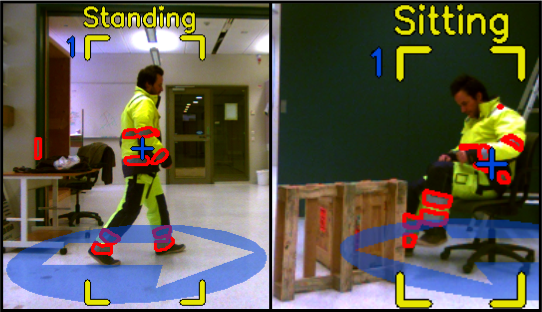
\includegraphics[width =1\linewidth]{figs/person_detection}
    % \vspace{-0.25cm}
    \caption{\textit{People detection:} (Left) the robot picks up an empty pallet in a designated
      zone; (Middle) the robot navigates to a loading zone where a can is detected and picked up;
      (Right) the loaded pallet is transported to a drop-off location.}
    \label{fig:people_det}
    \vspace{-0.5cm}
  \end{center}
\end{figure}
% 
As the envisioned mobile manipulation system will operate in environments shared with human workers,
people detection and human safety are important issues. In APPLE we address the problem by using the
RefleX system we recently developed~\cite{Mosb14}. RefleX is a camera-based on-board safety system
for industrial vehicles and machinery for detection of human workers wearing reflective vests worn
as per safety regulations. The system was designed with industrial safety standards in mind and is
currently being tested as an industrial prototype.
%

%
\section{Grasping and Manipulation}
\label{sec:manip}
%
\subsection{Grasp Planning}
\label{subsec:grasp_planning}
\begin{figure*}[t!] 
   \centering
    %\def\svgwidth{200pt} 
    \input{figs/grasp_interval.pdf_tex} 
   \caption{\textit{Grasp interval:} (Left) todo ... (Right) truncated grasp interval ...} 
   \label{fig:grasp_interval}
\end{figure*}

\cite{Bohg14}(data driven grasping) (SotA autonomous grasping systems) \cite{Pas13} cylinder shell
fitting

The key challenge for many applications of robotic mobile manipulation is autonomous grasping in
uncertain real-world environments. Finding collision-free trajec- tories leading the gripper-arm
chain from a given initial to a reachable final state (grasp planning together with vehicle and
manipulator motion planning) constitutes the fundament for any robot manipulation system. Currently,
despite of a large research effort, no commercially viable solution is available for this
problem. In today’s state-of-the-art autonomous grasping systems~\cite{Bere07, Srin10, Krug14a},
grasp planning and motion planning are usually seen as independent sub-problems~\cite{Dian10}. A
database storing object models together with pre-computed grasps is used to relax the need to find
suitable gripper poses/configurations~\cite{Mill04, Gold11, Krug14a}. In the online stage, sampling
based planners~\cite{LaVa06} attempt to generate valid trajectories for the pre-planned grasps,
which are executed in a feasible-first manner~\cite{Bere07}. During the execution phase, such
approaches necessitate many futile motion planning attempts, which often incurs significant time
delays since sampling based planners suffer from the curse of dimensionality. Also, while being able
to solve complicated planning problems if given enough time, these planners don’t scale well to
geometrically simple scenarios~\cite{Ratl09} and they are ill suited to incorporate contact events
with the environment.

 Instead of representing grasps as discrete gripper wrist poses and joint
configurations, we use grasp interval regions as depicted in Fig.~\ref{fig:grasp_interval}. These
grasp intervals can easily be transcribed as target tasks for the manipulator motion control and
allow for redundancy in the manipulator wrist positioning which eases reach-to-grasp
acquisition. Grasp interval formulation depends on the specific target object and has to be verified
experimentally. For now, we constrain ourselves to cylindrical objects as shown in
Fig.~\ref{fig:grasp_interval}. We then rely on the inherent capabilities of the grasping device and
the compliance of the system for successful grasp execution as stated below.


\cite{Bala12}(Identifying grasp principles from humans) \cite{Gien08a, Gien08b, Vahr10}(Task maps with RRT)
%
\subsection{Manipulator Motion Generation}
\label{subsec:manip_motion}
%
 \cite{Sams91}(task functions)
~\cite{Sici91, Sent10}(Redundant motion generation)

We follow the notation in~\cite{Esca14} and define the manipulator joint configuration by the vector
$\mbm{q}$ and the control inputs as corresponding joint velocities $\dot{\mbm{q}}$. A task function
is any derivable function of $\mbm{e}$. To give an example, a task with the purpose of bringing an
end-effector point $\mbm{p}(\mbm{q})$ onto a plane described by unit normal $\mbm{n}$ and offset $b$
can be transcribed by the task function $\mbm{e}=\mbm{n}^T\mbm{p}(\mbm{q})-d$ which formulates the
projection residual between the plane and $\mbm{p}(\mbm{q})$. The task evolution is given by
$\dot{\mbm{e}}=\mbm{J}\dot{\mbm{q}}$ with task jacobian
$\mbm{J}=\frac{\partial\mbm{e}}{\partial\mbm{q}}$.

Goal is to compute joint velocities such that the task evolution follows a desired reference profile
$\dot{\mbm{e}}^*$.

For reactive on-the-fly motion generation we formulate a stack of hierarchical tasks and use the
recently developed method by Kanoun et al.~\cite{Kano11}, which allows to account for inequality
tasks and solves a sequence of convex optimization problems at each time step to obtain
appropriate joint velocity commands (the method also can be used to directly generate torque
commands while accounting for the robot dynamics~\cite{Saab13}).
 
Obstacle avoidance is also achieved on a control-level, by formulating tasks which maintain minimum
distances between simple geometric primitives such as spheres, planes, points and capsules. We argue
that for the considered application strict collision avoidance is neither necessary nor desired,
since picking and manipulation inherently necessitates contact events between the robot and the
environment. Also, in real-world applications where knowledge about the environment is available
only in form of noisy sensor data, it might not be possible to avoid contacting the environment
without being overly conservative. This makes the KUKA LBR iiwa with its compliant low-level control
schemes and contact detection abilities an ideal platform for the tackled purpose and motion
generation scheme. The relatively simple picking task in APPLE provides an ideal testbed in a
real-world scenario.

\cite{Kano09}(Task function descriptions)
%
\subsection{Robust Grasp Execution}
\label{subsec:grasp_execution}
%
\begin{figure}[!t]
 \centering
   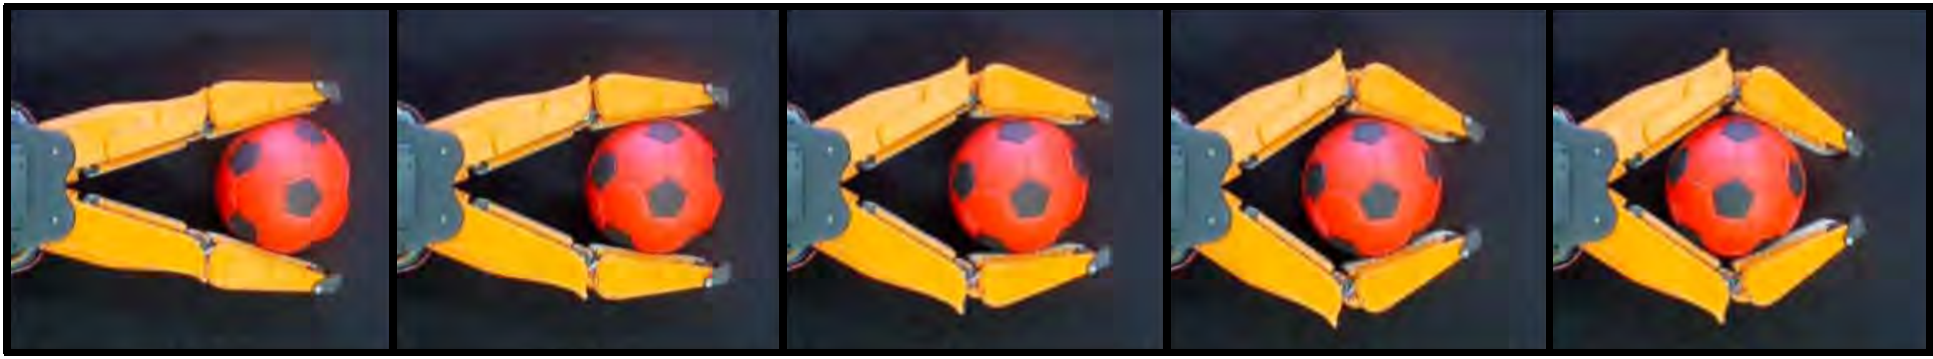
\includegraphics[width = 1.0\linewidth]{figs/pull_in}
   \caption{\textit{Pull-in grasping strategy:} Depicted is a sequence of intermediate grasp states
     where the belts of the gripper are used to pull the object towards its palm which results in a
     transition from a fingertip to an enveloping grasp.}
   \vspace{-4mm}
   \label{fig:pull_in}
   \centering
 \end{figure}
%
\begin{figure*}[!t]
 \centering
   \subfigure[]{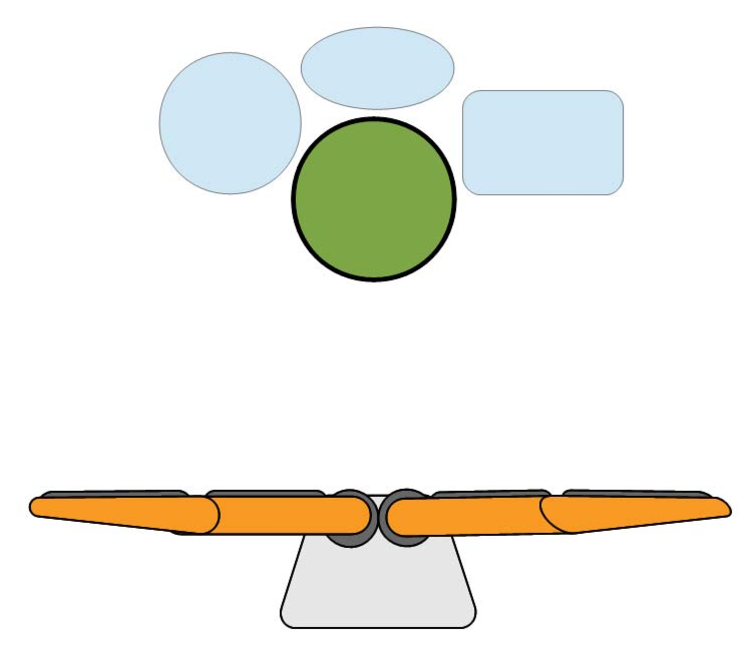
\includegraphics[width = .32\linewidth]{figs/vcg1}}
   \subfigure[]{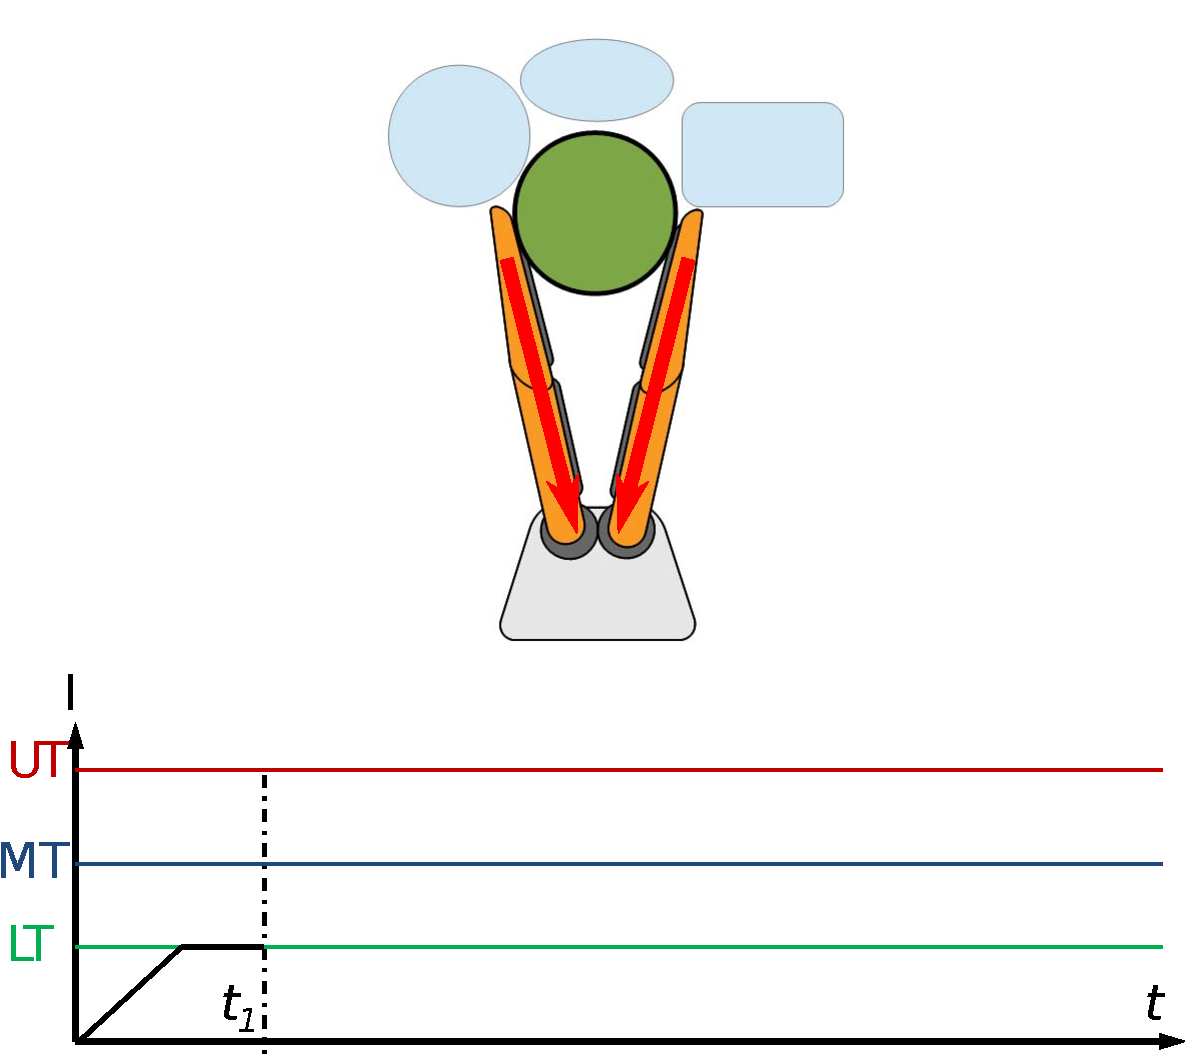
\includegraphics[width = .32\linewidth]{figs/vcg2}}
   \subfigure[]{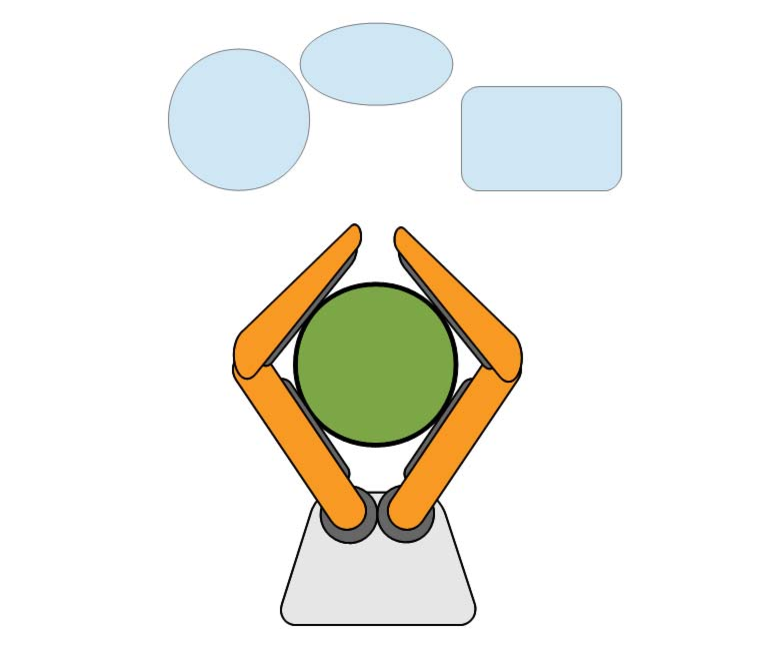
\includegraphics[width = .32\linewidth]{figs/vcg3}}
   \caption{\textit{Grasp Execution Control:} As the open griper closes in on the object (Left), the
     current through the opening motor is monitored. When contact is made (Middle), the actuated
     belts are switched on to pull in the object. The controller then strives to maintain the
     current in between two target thresholds by opening or closing the gripper during in-hand
     manipulation (Right).}
   \label{fig:pull_in_control}
 \centering
\end{figure*}
%
For this component, we leverage the capabilities of the Velvet Gripper, namely underactuation and
conveyor belts on the finger pads in order to achieve robust grasping behavior. Especially in
cluttered scenes, a ``pull-in'' strategy has been shown to be especially effective to achieve stable
grasps while starting from a relatively wide range of initial gripper poses with respect to the
target object~\cite{Krug14a}. Here, the features of the grasping device are exploited to embrace the
object in a firm envelope grasp by simultaneously squeezing it in a compliant fashion while
actuating the belts inwards.

(\hl{the following is copy/pasted from the Gripper control workshop paper})~\cite{Krug14c} Each of
the gripper’s two fingers has a planar manipulator structure with two joints and active surfaces
which are implemented by coupled conveyor belts on the inside of the two phalanges. The mechanical
structure is underactuated and comprises only one actuated Degree of Freedom (DoF) for opening and
closing and two DoF for the belt movements.  If, during grasping, the proximal phalanges are blocked
by an object, the gripper’s distal phalanges continue to “wrap around” and envelope it in a firm
grasp.  The experiments reported in~\cite{Krug14a} showed, that in cluttered scenes fingertip
grasps are more likely to be feasible than robust enveloping grasps, because the latter necessitate
large opening angles resulting in bulky gripper silhouettes for which no collision free approach
trajectories can be found. Therefore, we employ the “pull-in” strategy which is illustrated in
Fig.~\ref{nothereyet}. Here, the underactuated nature and the conveyor belts on the grasping device
are exploited to embrace the object in a firm envelope grasp by simultaneously squeezing it while
actuating the belts inwards. This is achieved by compliant low-level position controllers which
saturate on experimentally evaluated current thresholds. We use a simple grasping routine which is
triggered after an initial fingertip grasp is achieved (see Fig.~\ref{nothereyet}). This routine
consists of issuing commands to fully close the gripper while moving the belts a pre-defined offset
towards the palm. Three thresholds on the current absorption of the opening motor are used: a low
threshold (LT) signifies contact between the gripper and the object and a mid threshold (MT)
indicates a large enough contact force to stop the closing movement.  Finally, an upper threshold
(UT) prevents damage to the grasping device. Once the pull-in sequence is completed, the controllers
maintain the final torques to ensure a stable grasp.


%
\section{Evaluation}
\label{sec:eval}
% 
\begin{figure*}[t!]
  \begin{center}
    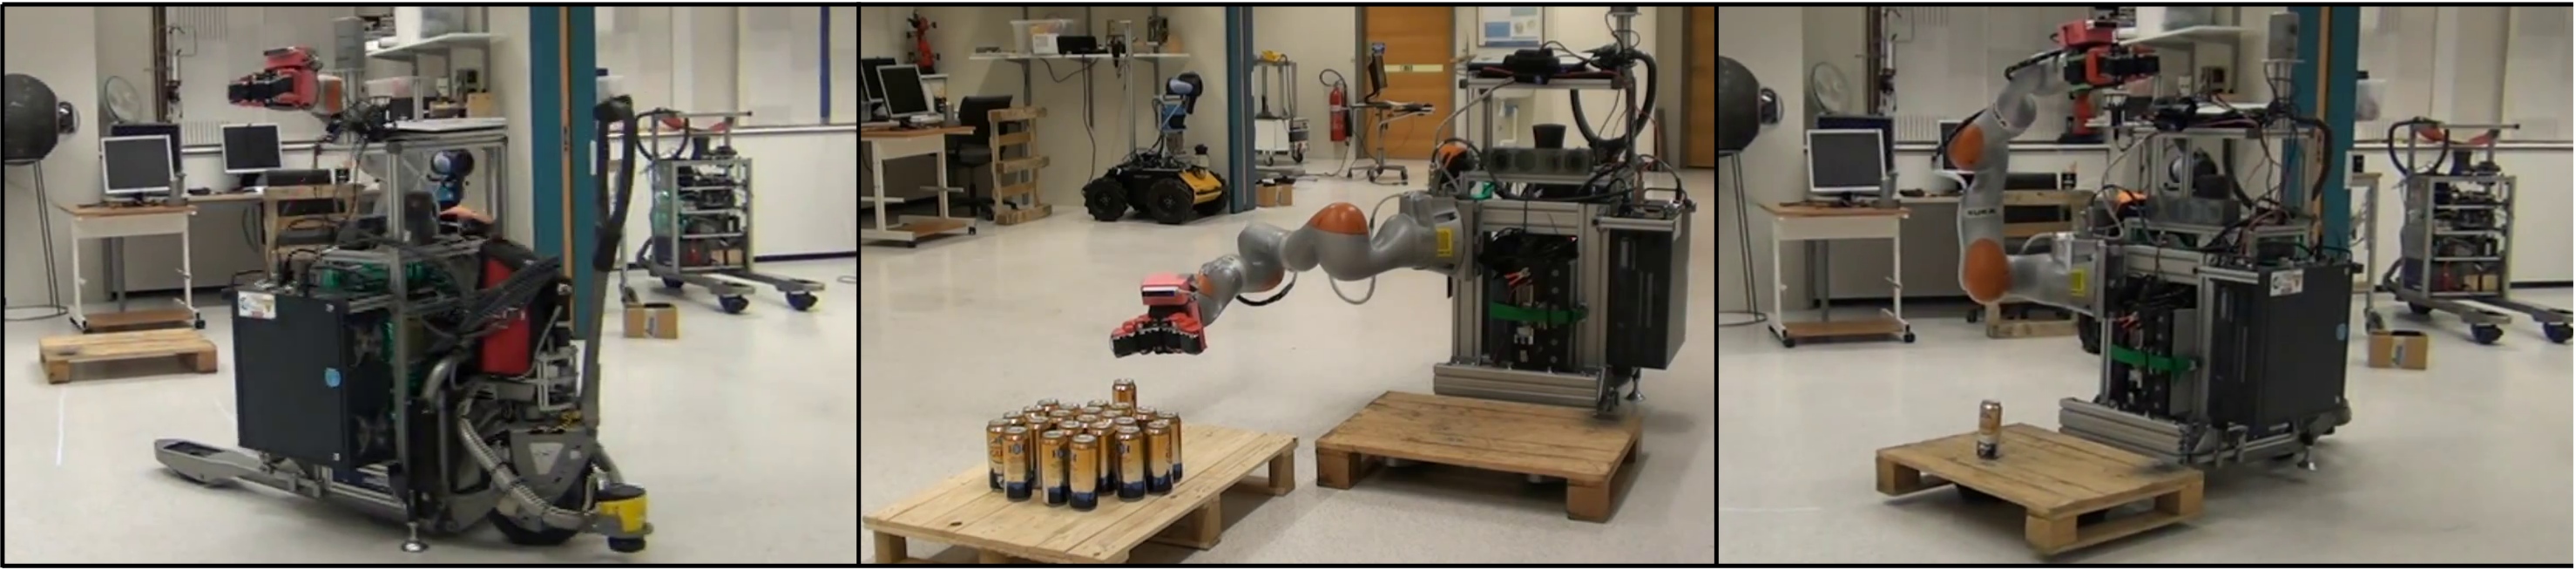
\includegraphics[width =1\linewidth]{figs/evaluation}
    % \vspace{-0.25cm}
    \caption{\textit{Evaluation setup:} (Left) the robot picks up an empty pallet in a designated
      zone; (Middle) the robot navigates to a loading zone where a can is detected and picked up;
      (Right) the loaded pallet is transported to a drop-off location.}
    \label{fig:evaluation}
    \vspace{-0.5cm}
  \end{center}
\end{figure*}
% 
For an early evaluation of the system, we set up a simplified commissioning scenario as depicted in
Fig.~\ref{fig:evaluation}. To this end, the previously described software components were
implemented in the Robot Operating System (ROS)~\cite{Quig09} framework. For manipulator motion
control (see Section~\ref{subsec:manip_motion}) we use the task function formulations
in~\cite{Kano09} for joint limit avoidance, obstacle avoidance and to formulate the inequality
constraints illustrated in Fig.~\ref{fig:truncated_grasp_interval} in order for the manipulator to
reach the grasp interval. An off-the-shelf solver~\cite{Guro15} is used to carry out the
optimizations for the motion control according to~\eqref{eq:HiQP}. As can be seen in the video
attachment to this article, we carried out successful trials at a run time of approximately 4
minutes for the whole procedure, of which 2 minutes were spent on object detection and grasping.




%
\section{Discussion and Outlook}
\label{sec:discussion}

\cite{Tass12}\cite{Kuma13}(optimal control for motion generation)

%
\section*{Acknowledgments}
%
The authors would like to thank Per Sporrong, Bo-Lennart Silfverdal, Bengt {\AA}sberg and Joakim
Larsson at {\"O}rebro University for their engineering support.
%
\bibliographystyle{IEEEtran}
\bibliography{References}

% \newpage
% REMARKS:
% \begin{itemize}
% \item cite the books stating that shifting of initial states is not a problem
% \end{itemize}

\end{document}



